\section{Introduction}

\subsection{Cross-DC Erasure Coding: Why Now?}

As the entire IT industry is rapidly moving to the cloud, more and more data
centers are being built all over the globe. The event that one of the data
centers will fail catastrophically becomes inevitable over time. In other words,
this is no longer a matter of ``if'', but rather ``when''. 
%{\em Designing for disasters}~\cite{keeton04designing} becomes essential and
Data stored in the
cloud have to be protected against catastrophic data center failure.

There have been a long line of prior work~\cite{oceanstore:asplos00,
  pond:fast13, hail:ccs09, racs:socc10, hu12nccloud} arguing for storing data
in erasure coded form, as opposed to replication, across geo-graphically
distributed data centers. Compared to geo-replication, cross-DC erasure coding
tolerates data center failure and ensures durability, while significantly
reduces storage cost. The same economic force that has driven cloud providers to
erasure code data within individual data centers naturally extends to the
cross-DC scenario.

Nevertheless, none of the cloud providers today offer options to erasure code
customer data across data centers. This is largely due to the prohibitive cost
of cross-DC network traffic. The reduction in storage cost comes to balance the
additional cost of inflated cross-DC network traffic, for both read/write during
normal operation and access/rebuild in the event of data center failure, as
discussed in detail in Section~\ref{sec:motivation}. Since the total cost of
storing customer data needs to cover both the storage and the cross-DC network
traffic, cross-DC erasure coding has not seen wide deployment yet.

%\begin{table}[thp]
%\centering
%\small
%\begin{tabular}{|l|c|c|}
%\hline
%TransAtlantic Cable             & FLAG Atlantic 1~\cite{bib:FA-1}   & MAREA~\cite{bib:MAREA1, bib:MAREA2}
%\\ \hline \hline
%Ready For Service               & 2001                              & 2017
%\\ \hline
%Cost (Billion)                  & 1.1                               & undisclosed
%\\ \hline
%Capacity                        & 10 Gbps                           & 160 Tbps
%\\ \hline \hline
%\end{tabular}
%\caption{Cross-DC bandwidth cost reducing by orders of magnitude.}
%\label{tab:mears}
%\end{table}

Fortunately, technological breakthroughs in wide area networking have dramatically reduced cross-DC bandwidth cost.
There are two key driving forces. 1) The erbium-doped fiber
amplifiers~\cite{mears1986low} make it practical to amplify a huge spectrum of
optical signal directly, without the need to convert to electrical signal.
2) Dense Wave Division Multiplexing (DWDM) is in turn enabled by the fiber
amplifiers, which can send 10+ terabits per second over single fiber~\cite{zhu2011112}.
Most recently, Facebook and Microsoft have teamed up to build $MAREA$, a new
fiber optic cable under the Atlantic Ocean that uses eight pairs of fiber optic
strands and will come online in 2017 with 160 Tbps capacity~\cite{bib:MAREA1, bib:MAREA2}.
In comparison, a transatlantic cable dated back in 2001 cost 1.1 billion dollars,
but had a mere capacity of 10 Gbps~\cite{bib:FA-1}.
Hence, MAREA represents over 10,000$\times$ bandwidth increase in less than two decades.
While the cost of MAREA remains undisclosed, it suffices
to say that cross-DC bandwidth cost has reduced by several orders of magnitude.
The significant cost reduction in cross-DC bandwidth is now
making cross-DC erasure coding economically attractive.

\comment{bib:MAREA1, http://www.wsj.com/articles/facebook-and-microsoft-to-build-fiber-optic-cable-across-atlantic-1464298853}
\comment{bib:MAREA2, http://www.usatoday.com/story/experience/2016/05/26/microsoft-facebook-undersea-cable-google-marea-amazon/84984882/}
\comment{bib:FA-1, https://en.wikipedia.org/wiki/Fiber-Optic_Link_Around_the_Globe}

\begin{figure}[tp]
\centering
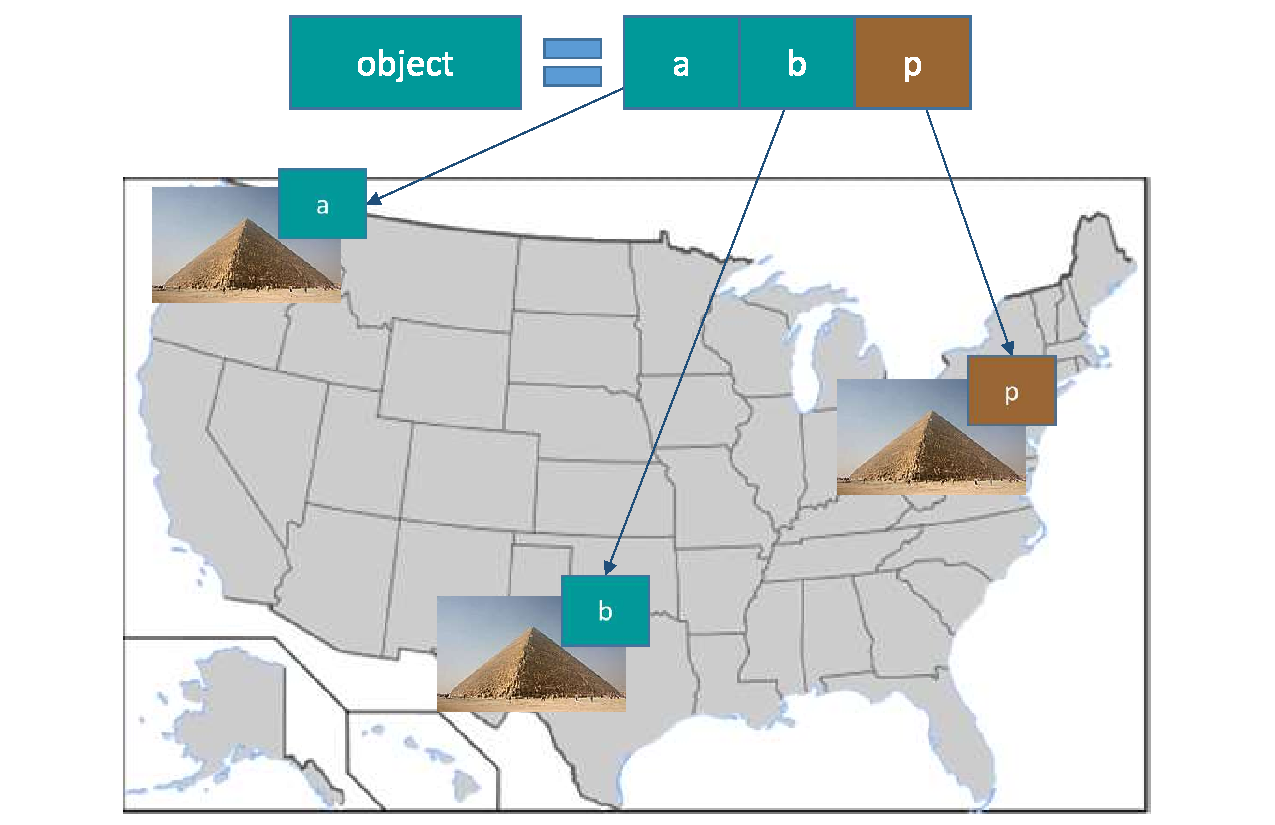
\includegraphics[width=0.4\textwidth]{images/giza_example_crop_fit}
\caption{Storing Object in Giza}
\label{fig:giza_example}
\end{figure}

\subsection{Giza Overview}

Giza exploits the reduction in cross-DC bandwidth cost
and leverages erasure coding to optimize the total cost of storing customer data in the cloud.
It offers an externally consistent (linearizable~\cite{herlihy90linearizability}),
versioned object store that erasure codes objects across global data centers.
Customers access Giza by creating Giza storage accounts. For each storage
account, the customers have the flexibility to choose the set of data centers
where their data are striped across. In addition, they can specify erasure coding scheme.
Giza employs classic $n = k + m$ Reed-Solomon coding, which generates $m$ parity fragments from $k$ data fragments.
All coded fragments are stored respectively in $n$ different DCs,
so as to tolerate up to $m$ arbitrary DC failures.
%By allowing the customers to choose the set of data centers and specify the erasure coding scheme, Giza gives the customers complete control of storage overhead and durability.
The customers access Giza with straightforward {\em put}, {\em get} and {\em delete} interface. In addition, Giza supports versioning, where new {\em put} does not overwrite existing data, but rather creates a new version of the same data. The old version remains available until it is explicitly deleted.

Giza operates on top of existing cloud storage systems that offers reliable and redudant local data storage. It stores data
objects in cloud blob storage and the metadata of the objects in cloud table
storage. Figure~\ref{fig:giza_example} illustrates an exemplary flow of storing
an object in Giza with 2 + 1 erasure coding.
%Giza operates a number of {\em stateless} Giza nodes in every data center. Say a customer uses a Giza client (command line, library, or REST interface) to store a 4MB data object. The Giza client routes the {\em put} request to one of the Giza nodes in the data center closest to the customer.
Giza divides the object into two data fragments ($a$ and $b$) and encodes them to a parity fragment $p$.
The fragments are stored respectively in the blob storage in three data centers. The metadata, consisting of the pointers to the
blobs, as well as versioning information, is replicated in the table storage across the
same data centers.

\subsection{Challenges and Contributions}

Giza targets cloud drive services which store predominantly large objects, such as
Dropbox, Google Drive, and Microsoft OneDrive, etc.
The design is motivated by the workload of such services observed in Section~\ref{sec:motivation}
and summarized here:
1) large storage space consumption,
2) cold data, where only a tiny percentage of objects are accessed
beyond a short period after creation,
3) objects may be updated over time, but concurrent updates of the same
object are rare (albeit possible).

Given the target workload, Giza optimizes for the common case, where there is
a single writer and multiple readers. Giza strives to {\em make the common case
fast}. In fact, the most optimized version of Giza achieves optimal latency,
which is a single cross-DC round trip for both {\em put} and {\em get}.

On the other hand, Giza handles the rare case properly,
and provides strong consistency when concurrent updates to the same object {\em do} occur.
%For instance, Giza tolerates data center failure. In the
%event of a data center being temporarily unavailable (or simply slow), the
%customers are able to continue to read and write data objects without much
%impact. The unavailable (or slow) data center may miss updates, which could
%potentially lead to conflict when they receive new updates again.
%For instance,
%the retry of a {\em put} could be processed by a different server (or even DC)
%and results in conflict with the previously unfinished {\em put}.
%Even though concurrency is rare,
%it is crucial for Giza to {\em guarantee the rare case correct}.
% Indeed, Giza provides external consistency.

Giza operates on top of existing cloud storage systems. 
The blob and table storage within individual data centers operate independently.
Hence, while strongly consistent individually, the collection of the blob and
table storage across multiple data centers do not readily offer the desired
external strong consistency. The key technical challenge Giza addresses is how to achieve
optimal latency with single {\em put}, while at the same time provide
strong consistency under concurrency, over the collection of individual blob and
table storage across multiple data centers.

Towards this end, the paper makes the following contributions:
\begin{itemize}
    \item We have designed and implemented Giza, a strongly consistent,
      versioned object store that erasure codes objects across globally
      distributed data centers.
    \item Giza is fast in the common case: when there is no concurrency, Giza
      completes within a single cross-DC round trip, which is optimal given the
      requirement to tolerate data center failure.
    \item Giza provides strong consistency when accessed concurrently, even with data center
      failure.
    \item Giza employs well-known distributed algorithms, such as Paxos and Fast
      Paxos, in a novel way so that it operates on top of existing cloud storage
      systems.
    \item Giza is deployed in xxx data centers. Experimental results demonstrate
      that Giza achieves all our design goals. In particular, it is worth
      pointing out that Giza achieves much lower latency than naively adopting a
      globally consistent storage system, like CockroachDB (widely considered as open source
      implementation of Google's Spanner).
\end{itemize}
